\chapter{Cristales I: el cristal perfecto y los metales}\label{ch:b1:crystals-metals}

Un hilo de cobre puede estirarse hasta ser más fino que un cabello sin
romperse; un terrón de sal se hace añicos bajo un martillo. Un herrero
calienta una barra de hierro hasta que brilla, la martillea, la sumerge en
agua, y la barra sale mucho más dura de lo que entró. La diferencia entre
estos comportamientos está en la manera en que se apilan los átomos del
sólido. La mayoría de los sólidos son \omterm{def:b1:crystals-metals:crystal}{cristales}: sus átomos se sitúan
según un patrón que se repite, idéntico, miles de millones de veces en
todas las direcciones. Este capítulo describe esos patrones, cuenta sus
átomos, mide lo apretados que están y dónde quedan los huecos entre
ellos, y usa el resultado para entender los metales y las aleaciones. El
capítulo siguiente aplica las mismas herramientas a los sólidos iónicos,
covalentes y moleculares.

\begin{recall}
Los metales pierden con facilidad sus \omterm{def:b1:quantum-numbers:configuration}{electrones de valencia}: tienen
energías de ionización y \omterm{def:b1:periodicity:electronegativity}{electronegatividades} bajas
(\cref{ch:b1:periodicity}). Los radios atómicos se definieron en la
\cref{def:b1:periodicity:radius}. La densidad, una propiedad que se
estudia en física, se da por conocida: $\rho = m/V$.
\end{recall}

\begin{omfigure}
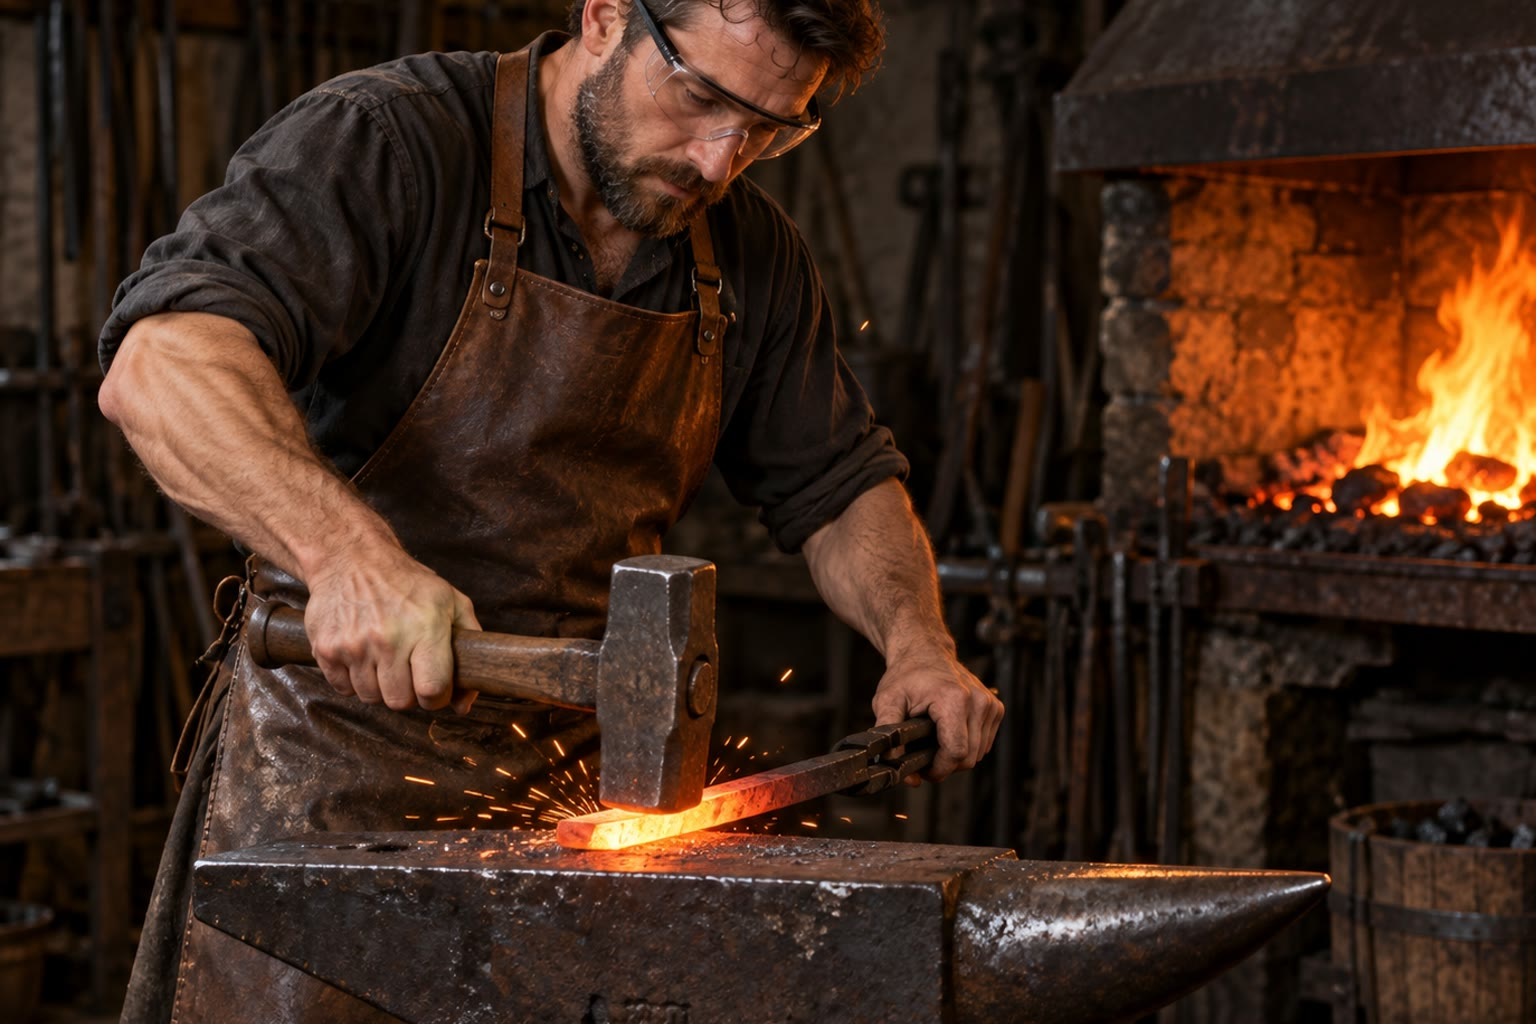
\includegraphics[width=0.55\linewidth]{images/book2/ai/b1-05-blacksmith.jpg}

{\small Un herrero forjando acero. El hierro que brilla en naranja tiene
una estructura cristalina distinta de la del hierro a temperatura
ambiente, y puede alojar más carbono (problema de fin de semana).}
\end{omfigure}

\section{El modelo del cristal perfecto}

\begin{definition}[Cristal, sólido amorfo, cristal perfecto]\label{def:b1:crystals-metals:crystal}
Un \emph{cristal}\index{cristal} es un sólido cuyas partículas (átomos,
iones o moléculas) están ordenadas según un patrón que se repite
periódicamente en las tres dimensiones. Un sólido sin ese orden de largo
alcance es un \emph{sólido amorfo}\index{solido amorfo@sólido amorfo} (el vidrio, la mayoría
de los plásticos). El \emph{modelo del cristal perfecto}\index{modelo del cristal perfecto}
describe un cristal como infinito y sin defectos: sin átomos que falten o
sobren, sin impurezas, sin fronteras.
\end{definition}

\begin{definition}[Red, motivo, celda unidad]\label{def:b1:crystals-metals:lattice}
Una \emph{red}\index{red} es un conjunto infinito de puntos, los
\emph{nodos}\index{nodo}, que se obtienen a partir de uno de ellos
mediante todas las traslaciones $u\,\vec a + v\,\vec b + w\,\vec c$ con
$u$, $v$,
$w$ enteros. El \omterm{def:b1:crystals-metals:crystal}{cristal} se obtiene colocando en cada nodo el mismo
\emph{motivo}\index{motivo} (un átomo, un grupo de átomos o de iones).
Una \emph{celda unidad}\index{celda unidad} es un paralelepípedo
construido sobre $\vec a$, $\vec b$, $\vec c$ cuyas traslaciones llenan el
espacio; las longitudes de sus aristas y sus ángulos son los
\emph{parámetros de red}\index{parametros de red@parámetros de red}
$a$, $b$, $c$, $\alpha$, $\beta$, $\gamma$. En una celda cúbica,
$a = b = c$ y los ángulos son de $90^\circ$.
\end{definition}

\begin{remark}[Los cristales reales]\label{rem:b1:crystals-metals:real}
Los \omterm{def:b1:crystals-metals:crystal}{cristales} reales son finitos e imperfectos: contienen vacantes,
impurezas, dislocaciones y límites de grano, que gobiernan muchas
propiedades (la ductilidad del cobre, la dureza del acero). Estos
defectos se estudian en el volumen del tercer año; el \omterm{def:b1:crystals-metals:crystal}{cristal} perfecto da
la geometría, la densidad y la \omterm{def:b1:crystals-metals:compactness}{compacidad}, que los defectos apenas
modifican.
\end{remark}

\begin{definition}[Multiplicidad de una celda]\label{def:b1:crystals-metals:multiplicity}
La \emph{multiplicidad}\index{multiplicidad} $Z$ de una celda es el número
de \omterm{def:b1:crystals-metals:lattice}{motivos} (o de átomos) que le pertenecen; cada átomo compartido con
las celdas vecinas cuenta por la fracción que queda dentro de ella.
\end{definition}

\begin{method}[Contar los átomos de una celda]\label{met:b1:crystals-metals:count}
En una celda cúbica, un átomo en un vértice lo comparten 8 celdas y
cuenta $1/8$; en una arista lo comparten 4 y cuenta $1/4$; en una cara lo
comparten 2 y cuenta $1/2$; en el interior cuenta 1. Se suman las
contribuciones.
\end{method}

\begin{definition}[Número de coordinación]\label{def:b1:crystals-metals:coordination}
El \emph{número de coordinación}\index{numero de coordinacion@número de coordinación} de una
partícula de un sólido es el número de sus vecinos más próximos, los que
están a la distancia más corta.
\end{definition}

\begin{definition}[Compacidad]\label{def:b1:crystals-metals:compactness}
La \emph{compacidad}\index{compacidad} (o fracción de empaquetamiento) de
un \omterm{def:b1:crystals-metals:crystal}{cristal} de esferas rígidas es la fracción del volumen que ocupan las
esferas: para una celda de volumen $V$ que contiene $Z$ esferas de radio
$R$,
\[
  C = \frac{Z \cdot \frac43 \pi R^3}{V} .
\]
\end{definition}

\begin{proposition}[Densidad a partir de la celda]\label{prop:b1:crystals-metals:density}
La densidad de un \omterm{def:b1:crystals-metals:crystal}{cristal} cuya celda, de volumen $V$, contiene $Z$
partículas de masa molar $M$ es
\[
  \rho = \frac{Z\,M}{N_A\,V} .
\]
\end{proposition}

\begin{proof}
La celda contiene $Z$ partículas, de masa $Z\,M/N_A$; el \omterm{def:b1:crystals-metals:crystal}{cristal} es la
celda repetida, de modo que su densidad es la de una celda.
\end{proof}

\section{Empaquetamientos compactos: cúbico centrado en las caras y hexagonal}

\begin{definition}[Empaquetamiento compacto, FCC, HCP]\label{def:b1:crystals-metals:packings}
Un \emph{empaquetamiento compacto}\index{empaquetamiento compacto} de
esferas iguales se construye con capas compactas, en las que cada esfera
toca a otras seis, apiladas de modo que cada esfera de una capa se apoya
en un hueco de la capa inferior. El apilamiento $ABCABC\dots$ da la
estructura \emph{cúbica centrada en las caras}\index{cubica centrada en las caras@cúbica centrada en las caras}
(FCC, o cúbica compacta); el apilamiento $ABAB\dots$ da la estructura
\emph{hexagonal compacta}\index{hexagonal compacta} (HCP). Una tercera
estructura de los metales, no compacta, es la \emph{cúbica centrada en el
cuerpo}\index{cubica centrada en el cuerpo@cúbica centrada en el cuerpo} (BCC), un cubo con un átomo en cada vértice y otro en su
centro.
\end{definition}

\begin{omfigure}
\begin{tikzpicture}[font=\small]
  % layer A
  \foreach \i in {0,...,4} \foreach \j in {0,...,3} {
    \pgfmathsetmacro\x{\i+0.5*\j}
    \pgfmathsetmacro\y{0.866*\j}
    \draw[black!60, fill=omDef!25] (\x,\y) circle (0.5);
  }
  % layer B, in the hollows pointing up
  \foreach \i/\j in {1/0, 2/0, 3/0, 1/1, 2/1, 3/1, 1/2, 2/2} {
    \pgfmathsetmacro\x{\i+0.5*\j}
    \pgfmathsetmacro\y{0.866*\j+0.577}
    \draw[omThm!80!black, fill=omThm!25, fill opacity=0.75] (\x,\y) circle (0.5);
  }
  % C positions
  \foreach \i/\j in {1/0, 2/0, 3/0, 1/1, 2/1, 3/1} {
    \pgfmathsetmacro\x{\i+0.5+0.5*\j}
    \pgfmathsetmacro\y{0.866*\j+0.289}
    \fill[omMeth] (\x,\y) circle (0.11);
  }
  \node[anchor=west, align=left] at (6.6,1.6) {A: primera capa (azul)\\B: segunda capa, en los\\\phantom{B: }huecos de A (rojo)\\C: los otros huecos\\\phantom{C: }(puntos verdes)};
\end{tikzpicture}

{\small Dos capas compactas vistas desde arriba. Una tercera capa puede
colocarse sobre los huecos marcados C (apilamiento $ABC$, \omterm{def:b1:crystals-metals:packings}{cúbica centrada
en las caras}) o sobre los átomos de A (apilamiento $AB$, \omterm{def:b1:crystals-metals:packings}{hexagonal
compacta}).}
\end{omfigure}

\begin{proposition}[Cúbica centrada en las caras]\label{prop:b1:crystals-metals:fcc}
En la estructura FCC, los átomos ocupan los ocho vértices y los seis
centros de las caras de un cubo de arista $a$. Entonces, $Z = 4$, el
\omterm{def:b1:crystals-metals:coordination}{número de coordinación} es 12, los átomos se tocan a lo largo de una
diagonal de cara, $a\sqrt2 = 4R$, y la \omterm{def:b1:crystals-metals:compactness}{compacidad} es
\[
  C = \frac{\pi}{3\sqrt2} \approx 0.74 .
\]
\end{proposition}

\begin{proof}
$Z = 8 \times \frac18 + 6 \times \frac12 = 4$. Un átomo del centro de una
cara toca los cuatro vértices de su cara y los cuatro centros de cara de
cada una de las dos celdas que comparten la cara: $4 + 4 + 4 = 12$
vecinos a $a\sqrt2/2$. Sobre una diagonal de cara, de longitud
$a\sqrt2$, hay un átomo de vértice, uno de centro de cara y otro de
vértice en contacto: $a\sqrt2 = 4R$. Entonces,
$C = 4 \cdot \frac43\pi R^3/a^3 = \frac{16}{3}\pi R^3/(2\sqrt2 R)^3 \cdot
\frac{1}{1} = \frac{16\pi}{3 \times 16\sqrt2} = \frac{\pi}{3\sqrt2}$.
\end{proof}

\begin{omfigure}
\tdplotsetmaincoords{60}{100}
\begin{tikzpicture}[tdplot_main_coords, font=\small]
  \pic {omcubeo={3}};
  \node[cellA=6mm] at (0,0,0) {};
  \node[cellA=6mm] at (0,3,0) {};
  \node[cellA=6mm, ball color=omDef!55] at (0,1.5,1.5) {};
  \node[cellA=6mm] at (0,0,3) {};
  \node[cellA=6mm, ball color=omDef!55] at (1.5,1.5,0) {};
  \node[cellA=6mm] at (0,3,3) {};
  \node[cellA=6mm, ball color=omDef!55] at (1.5,0,1.5) {};
  \node[cellA=6mm, ball color=omDef!55] at (1.5,3,1.5) {};
  \node[cellA=6mm] at (3,0,0) {};
  \node[cellA=6mm, ball color=omDef!55] at (1.5,1.5,3) {};
  \node[cellA=6mm] at (3,3,0) {};
  \node[cellA=6mm, ball color=omDef!55] at (3,1.5,1.5) {};
  \node[cellA=6mm] at (3,0,3) {};
  \node[cellA=6mm] at (3,3,3) {};
  \draw[omThm, thick] (3,0,0) -- (3,3,3);
\end{tikzpicture}
\hspace{1.2cm}
\begin{tikzpicture}[tdplot_main_coords, font=\small]
  \pic {omcubeo={3}};
  \node[cellA=7mm] at (0,0,0) {};
  \node[cellA=7mm] at (0,3,0) {};
  \node[cellA=7mm] at (0,0,3) {};
  \node[cellA=7mm] at (0,3,3) {};
  \node[cellA=7mm, ball color=omDef!55] at (1.5,1.5,1.5) {};
  \node[cellA=7mm] at (3,0,0) {};
  \node[cellA=7mm] at (3,3,0) {};
  \node[cellA=7mm] at (3,0,3) {};
  \node[cellA=7mm] at (3,3,3) {};
  \draw[omThm, thick] (3,0,0) -- (0,3,3);
\end{tikzpicture}

{\small A la izquierda, la celda \omterm{def:b1:crystals-metals:packings}{cúbica centrada en las caras} (átomos de
los vértices en gris, de los centros de cara en azul). Los átomos se
tocan a lo largo de una diagonal de cara (línea roja, $a\sqrt2 = 4R$). A
la derecha, la celda \omterm{def:b1:crystals-metals:packings}{cúbica centrada en el cuerpo}; los átomos se tocan a
lo largo de la diagonal principal (línea roja, $a\sqrt3 = 4R$).
Para mayor claridad, los átomos se dibujan más pequeños que su tamaño de
contacto.}
\end{omfigure}

\begin{proposition}[Hexagonal compacta]\label{prop:b1:crystals-metals:hcp}
En la estructura HCP, el prisma hexagonal convencional, de arista de base
$a$ y altura $c$, contiene 6 átomos; el \omterm{def:b1:crystals-metals:coordination}{número de coordinación} es 12; para
esferas en contacto, $a = 2R$, $c/a = \sqrt{8/3} \approx 1.633$, y la
\omterm{def:b1:crystals-metals:compactness}{compacidad} es la misma que en la FCC, $\pi/(3\sqrt2) \approx 0.74$.
\end{proposition}

\begin{proof}
El prisma tiene 12 átomos de vértice compartidos por 6 prismas, 2 átomos
de centro de cara compartidos por 2 y 3 átomos interiores:
$12/6 + 2/2 + 3 = 6$. Cada átomo toca seis vecinos en su capa y tres en
cada capa adyacente: 12. Un átomo de la capa B se apoya en tres átomos en
contacto de la capa A, formando un tetraedro regular de arista $2R$, cuya
altura es $2R\sqrt{2/3}$; dos capas más arriba, $c = 4R\sqrt{2/3}$, de
modo que $c/a = 2\sqrt{2/3} = \sqrt{8/3}$. El volumen del prisma es
$\frac{3\sqrt3}{2}a^2 c = \frac{3\sqrt3}{2}(2R)^2 \cdot
4R\sqrt{2/3} = 24\sqrt2\,R^3$, y $C = 6 \cdot \frac43\pi R^3/(24\sqrt2
R^3) = \pi/(3\sqrt2)$.
\end{proof}

\begin{omfigure}
\tdplotsetmaincoords{70}{113}
\begin{tikzpicture}[tdplot_main_coords, font=\small, scale=1.25]
  \pic[transform shape] {omhexprismo={1.6}{2.6}};
  \node[cellA=6mm] at (-1.6,0,0) {};
  \node[cellA=6mm] at (-0.8,-1.386,0) {};
  \node[cellA=6mm] at (-1.6,0,2.6) {};
  \node[cellA=6mm] at (-0.8,-1.386,2.6) {};
  \node[cellA=6mm] at (-0.8,1.386,0) {};
  \node[cellA=6mm, ball color=omThm!60] at (-0.8,0.462,1.3) {};
  \node[cellA=6mm] at (0,0,0) {};
  \node[cellA=6mm, ball color=omThm!60] at (0,-0.924,1.3) {};
  \node[cellA=6mm] at (0.8,-1.386,0) {};
  \node[cellA=6mm] at (-0.8,1.386,2.6) {};
  \node[cellA=6mm] at (0,0,2.6) {};
  \node[cellA=6mm] at (0.8,-1.386,2.6) {};
  \node[cellA=6mm] at (0.8,1.386,0) {};
  \node[cellA=6mm, ball color=omThm!60] at (0.8,0.462,1.3) {};
  \node[cellA=6mm] at (1.6,0,0) {};
  \node[cellA=6mm] at (0.8,1.386,2.6) {};
  \node[cellA=6mm] at (1.6,0,2.6) {};
\end{tikzpicture}

{\small El prisma hexagonal compacto, de arista de base $a$ (el lado del
hexágono) y altura $c$: capas A (gris) abajo y arriba, y capa B (roja) a
media altura, alojada en los huecos de A.}
\end{omfigure}

\section{La cúbica centrada en el cuerpo y los elementos metálicos}

\begin{proposition}[Cúbica centrada en el cuerpo]\label{prop:b1:crystals-metals:bcc}
En la estructura BCC, $Z = 2$, el \omterm{def:b1:crystals-metals:coordination}{número de coordinación} es 8, los átomos
se tocan a lo largo de la diagonal principal del cubo, $a\sqrt3 = 4R$, y
la \omterm{def:b1:crystals-metals:compactness}{compacidad} es
\[
  C = \frac{\pi\sqrt3}{8} \approx 0.68 .
\]
\end{proposition}

\begin{proof}
$Z = 8 \times \frac18 + 1 = 2$. El átomo central toca los ocho vértices:
la diagonal principal $a\sqrt3$ contiene un vértice, el centro y otro
vértice, $a\sqrt3 = 4R$. Entonces, $C = 2 \cdot \frac43\pi R^3/a^3 =
\frac83\pi R^3 (\sqrt3/(4R))^3 = \frac83\pi \cdot \frac{3\sqrt3}{64} =
\frac{\pi\sqrt3}{8}$.
\end{proof}

\begin{proposition}[El empaquetamiento compacto es el más denso]\label{prop:b1:crystals-metals:kepler}
Ningún empaquetamiento de esferas iguales tiene una \omterm{def:b1:crystals-metals:compactness}{compacidad} mayor que
$\pi/(3\sqrt2) \approx 0.7405$, el valor de las estructuras FCC y HCP.
\end{proposition}
\admitted

\begin{history}[La conjetura de Kepler, 1611--2017]
En un breve ensayo sobre los copos de nieve, escrito en 1611, Johannes
Kepler afirmó que ninguna manera de apilar balas de cañón podía ser más
densa que la pirámide del frutero, el empaquetamiento cúbico centrado en
las caras. El enunciado resistió la demostración durante casi cuatro
siglos. Thomas Hales dio una demostración asistida por ordenador en 1998,
y en 2014 se completó una demostración formal, verificada línea a línea
por ordenador, que se publicó en 2017.
\end{history}

\begin{example}[Tres metales]\label{ex:b1:crystals-metals:metals}
El cobre es FCC con $a = \qty{361.5}{pm}$: $R = a\sqrt2/4 =
\qty{127.8}{pm}$ y $\rho = 4 \times 63.55/(6.022 \times 10^{23} \times
(3.615 \times 10^{-8})^3) = \qty{8.93}{g/cm^3}$, la densidad medida. El
hierro a temperatura ambiente (hierro $\alpha$) es BCC con
$a = \qty{286.7}{pm}$: $R = \qty{124.1}{pm}$, $\rho = \qty{7.87}{g/cm^3}$.
El magnesio es HCP con $a = \qty{320.9}{pm}$ y $c = \qty{521.0}{pm}$:
$c/a = 1.624$, próximo al ideal, $1.633$; el cinc, con $c/a = 1.856$, es
un empaquetamiento hexagonal alargado.
% ledger: lat:Cu, rho:Cu, lat:Fe-alpha, rho:Fe, lat:Mg.a, lat:Mg.c,
% lat:Zn.a, lat:Zn.c, aw:Cu, aw:Fe, const:NA
\end{example}

\begin{center}
\small
\begin{tabular}{lllccc}
\hline
metal & estructura & $a$ (pm) & $R$ (pm) & $\rho$ calculada & $\rho$ medida \\
\hline
aluminio & FCC & 405.0 & 143.2 & 2.70 & 2.70 \\
cobre & FCC & 361.5 & 127.8 & 8.93 & 8.93 \\
plata & FCC & 408.6 & 144.5 & 10.50 & 10.50 \\
sodio & BCC & 429.1 & 185.8 & 0.967 & 0.97 \\
hierro $\alpha$ & BCC & 286.7 & 124.1 & 7.87 & 7.87 \\
wolframio & BCC & 316.5 & 137.0 & 19.26 & 19.3 \\
\hline
\end{tabular}
\end{center}
% ledger: lat:Al, lat:Cu, lat:Ag, lat:Na, lat:Fe-alpha, lat:W, rho:Al,
% rho:Cu, rho:Ag, rho:Na, rho:Fe, rho:W (densities in g/cm3)

\begin{omfigure}
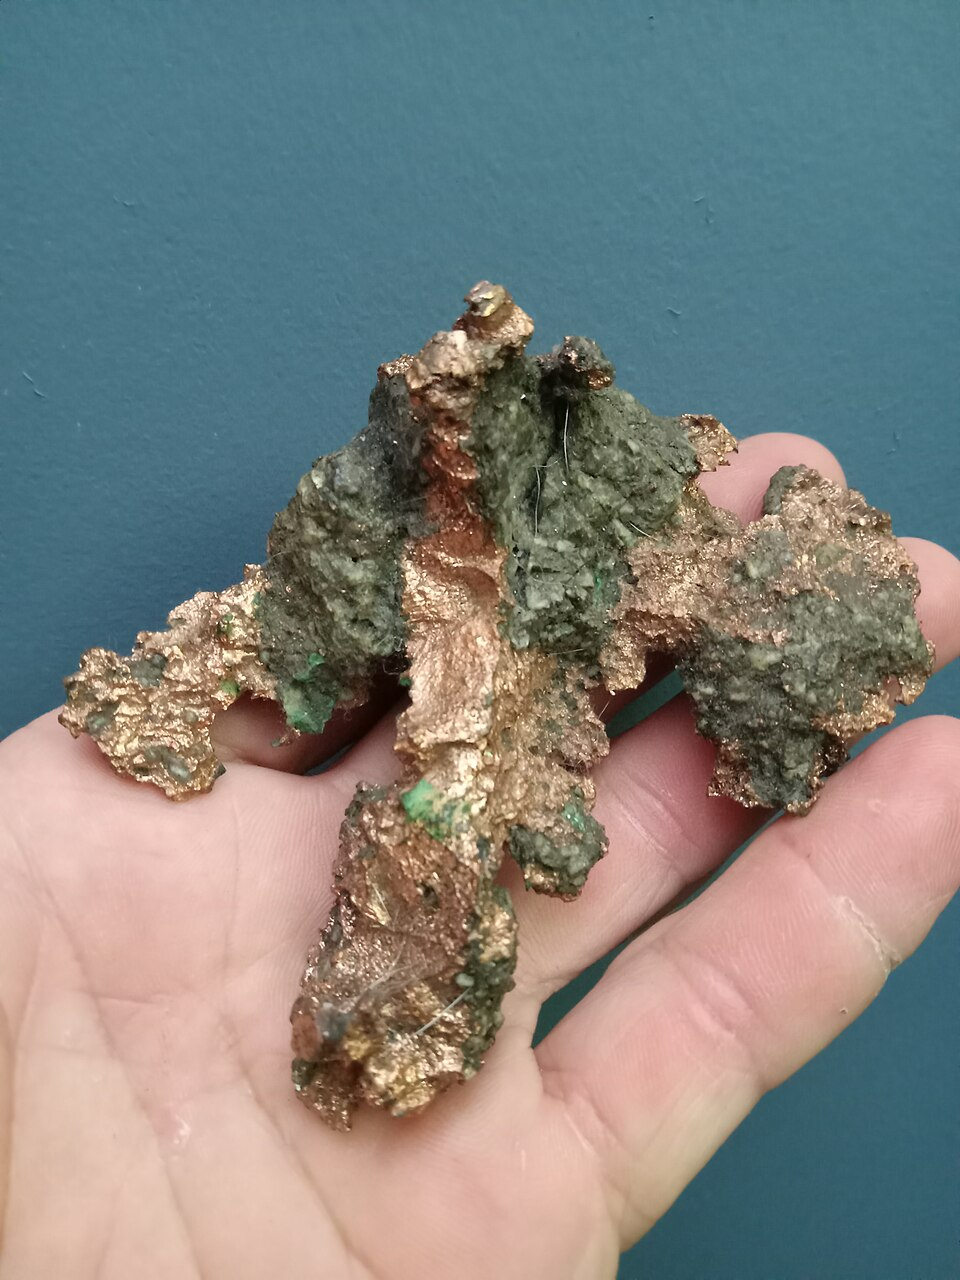
\includegraphics[width=0.36\linewidth]{images/book2/native-copper.jpg}

{\small Un ejemplar de cobre nativo. Sus formas ramificadas crecieron como
\omterm{def:b1:crystals-metals:crystal}{cristales}; el metal es por dentro un mosaico de granos FCC.
Foto: CC0 (Wikimedia Commons).}
\end{omfigure}

\section{Huecos intersticiales}

\begin{definition}[Huecos intersticiales]\label{def:b1:crystals-metals:site}
Un \emph{hueco intersticial}\index{hueco intersticial} es un espacio entre
los átomos de un \omterm{def:b1:crystals-metals:crystal}{cristal} donde puede alojarse un átomo más pequeño. Un
\emph{hueco tetraédrico}\index{hueco tetraedrico@hueco tetraédrico} está en el centro de un
tetraedro de cuatro átomos, y un \emph{hueco octaédrico}\index{hueco octaedrico@hueco octaédrico}, en el
centro de un octaedro de seis. El \emph{radio del hueco}\index{radio del hueco}
es el radio de la mayor esfera que cabe en él sin separar los átomos que
lo rodean.
\end{definition}

\begin{proposition}[Huecos de la estructura FCC]\label{prop:b1:crystals-metals:sites}
Una celda FCC contiene 4 \omterm{def:b1:crystals-metals:site}{huecos octaédricos}, en el centro del cubo y en
los puntos medios de sus 12 aristas, y 8 \omterm{def:b1:crystals-metals:site}{huecos tetraédricos}, en los
centros de los 8 cubos pequeños de arista $a/2$. Para átomos de radio $R$
en contacto, los radios de los huecos son
\[
  r_O = (\sqrt2 - 1)R \approx 0.414\,R, \qquad
  r_T = \left(\sqrt{\tfrac32} - 1\right)R \approx 0.225\,R .
\]
\end{proposition}

\begin{proof}
\omterm{def:b1:crystals-metals:site}{Huecos octaédricos}: $1 + 12 \times \frac14 = 4$, tantos como átomos. El
centro del cubo está a $a/2$ de los seis centros de cara: $r_O + R = a/2$
con $a = 2\sqrt2 R$, de modo que $r_O = (\sqrt2 - 1)R$. \omterm{def:b1:crystals-metals:site}{Huecos
tetraédricos}: el centro de un cubo pequeño de arista $a/2$ está a la
mitad de su diagonal principal,
$\frac{a}{2}\cdot\frac{\sqrt3}{2} = \frac{a\sqrt3}{4}$, de los cuatro
átomos situados en vértices alternos: $r_T + R = \frac{\sqrt3}{4}\,2\sqrt2\,R =
\sqrt{\tfrac32}\,R$.
\end{proof}

\begin{omfigure}
\tdplotsetmaincoords{60}{100}
\begin{tikzpicture}[tdplot_main_coords, font=\small]
  \pic {omcubeo={3}};
  \node[cellA=3.6mm] at (0,0,0) {};
  \node[cellsite=4mm, draw=omThm, fill=omThm!30] at (0,1.5,0) {};
  \node[cellA=3.6mm] at (0,3,0) {};
  \node[cellsite=4mm, draw=omThm, fill=omThm!30] at (0,0,1.5) {};
  \node[cellA=3.6mm] at (0,1.5,1.5) {};
  \node[cellsite=4mm, draw=omThm, fill=omThm!30] at (0,3,1.5) {};
  \node[cellsite=4mm, draw=omThm, fill=omThm!30] at (1.5,0,0) {};
  \node[cellA=3.6mm] at (0,0,3) {};
  \node[cellA=3.6mm] at (1.5,1.5,0) {};
  \node[cellsite=4mm, draw=omThm, fill=omThm!30] at (0,1.5,3) {};
  \node[cellsite=4mm, draw=omThm, fill=omThm!30] at (1.5,3,0) {};
  \node[cellA=3.6mm] at (0,3,3) {};
  \node[cellA=3.6mm] at (1.5,0,1.5) {};
  \node[cellsite=5mm, draw=omThm, fill=omThm!30] at (1.5,1.5,1.5) {};
  \node[cellA=3.6mm] at (1.5,3,1.5) {};
  \node[cellA=3.6mm] at (3,0,0) {};
  \node[cellsite=4mm, draw=omThm, fill=omThm!30] at (1.5,0,3) {};
  \node[cellsite=4mm, draw=omThm, fill=omThm!30] at (3,1.5,0) {};
  \node[cellA=3.6mm] at (1.5,1.5,3) {};
  \node[cellA=3.6mm] at (3,3,0) {};
  \node[cellsite=4mm, draw=omThm, fill=omThm!30] at (1.5,3,3) {};
  \node[cellsite=4mm, draw=omThm, fill=omThm!30] at (3,0,1.5) {};
  \node[cellA=3.6mm] at (3,1.5,1.5) {};
  \node[cellsite=4mm, draw=omThm, fill=omThm!30] at (3,3,1.5) {};
  \node[cellA=3.6mm] at (3,0,3) {};
  \node[cellsite=4mm, draw=omThm, fill=omThm!30] at (3,1.5,3) {};
  \node[cellA=3.6mm] at (3,3,3) {};
  \node[below] at (1.5,1.5,-1.5) {huecos octaédricos (rojo)};
\end{tikzpicture}
\hspace{1.2cm}
\begin{tikzpicture}[tdplot_main_coords, font=\small]
  \pic {omcubeo={3}};
  \node[cellA=3.6mm] at (0,0,0) {};
  \node[cellA=3.6mm] at (0,3,0) {};
  \node[cellA=3.6mm] at (0,1.5,1.5) {};
  \node[cellsite=4mm, fill=omDef!30] at (0.75,0.75,0.75) {};
  \node[cellsite=4mm, fill=omDef!30] at (0.75,2.25,0.75) {};
  \node[cellA=3.6mm] at (0,0,3) {};
  \node[cellA=3.6mm] at (1.5,1.5,0) {};
  \node[cellsite=4mm, fill=omDef!30] at (0.75,0.75,2.25) {};
  \node[cellA=3.6mm] at (0,3,3) {};
  \node[cellA=3.6mm] at (1.5,0,1.5) {};
  \node[cellsite=4mm, fill=omDef!30] at (0.75,2.25,2.25) {};
  \node[cellsite=4mm, fill=omDef!30] at (2.25,0.75,0.75) {};
  \node[cellA=3.6mm] at (1.5,3,1.5) {};
  \node[cellA=3.6mm] at (3,0,0) {};
  \node[cellsite=4mm, fill=omDef!30] at (2.25,2.25,0.75) {};
  \node[cellA=3.6mm] at (1.5,1.5,3) {};
  \node[cellA=3.6mm] at (3,3,0) {};
  \node[cellsite=4mm, fill=omDef!30] at (2.25,0.75,2.25) {};
  \node[cellsite=4mm, fill=omDef!30] at (2.25,2.25,2.25) {};
  \node[cellA=3.6mm] at (3,1.5,1.5) {};
  \node[cellA=3.6mm] at (3,0,3) {};
  \node[cellA=3.6mm] at (3,3,3) {};
  \draw[omDef!70!black, thin] (0,0,0) -- (0.75,0.75,0.75) -- (1.5,1.5,0)
    (0.75,0.75,0.75) -- (1.5,0,1.5) (0.75,0.75,0.75) -- (0,1.5,1.5);
  \node[below] at (1.5,1.5,-1.5) {huecos tetraédricos (azul)};
\end{tikzpicture}

{\small \omterm{def:b1:crystals-metals:site}{Huecos intersticiales} de la celda FCC. A la izquierda, el \omterm{def:b1:crystals-metals:site}{hueco
octaédrico} del centro y los de los puntos medios de las aristas
(compartidos por cuatro celdas). A la derecha, los ocho \omterm{def:b1:crystals-metals:site}{huecos
tetraédricos} en los centros de los octavos del cubo, uno de ellos unido a
sus cuatro átomos.}
\end{omfigure}

\section{El enlace metálico y las aleaciones}

\begin{definition}[Enlace metálico]\label{def:b1:crystals-metals:metallic-bond}
En el \emph{enlace metálico}\index{enlace metalico@enlace metálico}, cada átomo de un metal
cede sus \omterm{def:b1:quantum-numbers:configuration}{electrones de valencia} a todo el \omterm{def:b1:crystals-metals:crystal}{cristal}: el sólido es una \omterm{def:b1:crystals-metals:lattice}{red}
de cationes bañados en electrones que no pertenecen a ningún átomo en
particular y se mueven libremente por él. El enlace es la atracción entre
los cationes y esta nube de electrones compartida; no es direccional.
\end{definition}

\begin{proposition}[Propiedades de los metales]\label{prop:b1:crystals-metals:properties}
El \omterm{def:b1:crystals-metals:metallic-bond}{enlace metálico} explica las propiedades de los metales: los electrones
móviles conducen la electricidad y el calor y reflejan la luz (brillo);
como el enlace no es direccional, las capas de átomos pueden deslizarse
unas sobre otras sin que el \omterm{def:b1:crystals-metals:crystal}{cristal} se rompa (ductilidad, maleabilidad),
y los \omterm{def:b1:crystals-metals:packings}{empaquetamientos compactos}, que maximizan el número de vecinos, son
las estructuras más frecuentes.
\end{proposition}
\admitted

\begin{definition}[Aleaciones]\label{def:b1:crystals-metals:alloy}
Una aleación es un sólido metálico formado por varios elementos. En una
\emph{aleación de sustitución}\index{aleacion de sustitucion@aleación de sustitución} los átomos del elemento
añadido reemplazan átomos del anfitrión en su \omterm{def:b1:crystals-metals:lattice}{red}; esto exige radios que
no difieran en más de un 15\,\% aproximadamente (cobre y níquel, cobre y
cinc en el latón). En una \emph{aleación intersticial}\index{aleacion intersticial@aleación intersticial}
átomos pequeños (\ce{H}, \ce{C}, \ce{N}, \ce{B}) ocupan \omterm{def:b1:crystals-metals:site}{huecos
intersticiales} del anfitrión (el carbono en el acero).
\end{definition}

\begin{definition}[Alotropía]\label{def:b1:crystals-metals:allotropy}
Las distintas estructuras cristalinas de un mismo elemento son sus
\emph{alótropos}\index{alotropo@alótropo}. El hierro es BCC (hierro $\alpha$) a
temperatura ambiente; se ha medido FCC (hierro $\gamma$) de
\qty{1189}{K} a \qty{1661}{K}, y de nuevo BCC (hierro $\delta$) a
\qty{1662}{K}, hasta su punto de fusión. El carbono existe como diamante y
como grafito
(\cref{ch:b1:crystals-ionic-covalent}).
% ledger: lat:Fe-alpha, lat:Fe-gamma-1189, lat:Fe-gamma-1661,
% lat:Fe-delta-1662
\end{definition}

\begin{example}[El acero]\label{ex:b1:crystals-metals:steel}
El carbono, de \omterm{def:b1:periodicity:radius}{radio covalente} \qty{77}{pm} (la mitad de la distancia
\ce{C-C} en el diamante), es demasiado grande para los huecos del hierro
sin deformarlos, pero mucho menos en el hierro $\gamma$, cuyos \omterm{def:b1:crystals-metals:site}{huecos
octaédricos} son los mayores. El acero se fabrica disolviendo carbono en
hierro $\gamma$ caliente; al templarlo, el carbono queda atrapado
mientras el hierro vuelve a una estructura centrada en el cuerpo, que
deforma, y el \omterm{def:b1:crystals-metals:crystal}{cristal} deformado es duro.
% ledger: lat:C-diamond (r = a sqrt3 / 8 = 77.2 pm)
\end{example}

\begin{remark}[Las transiciones del hierro]\label{rem:b1:crystals-metals:iron-T}
Las temperaturas de la \cref{def:b1:crystals-metals:allotropy} son las del
hierro puro a presión atmosférica; el carbono disuelto rebaja la
temperatura a la que se forma el hierro $\gamma$, lo que hace trabajable
el acero. Los diagramas de fases de las aleaciones se estudian en el
volumen del segundo año.
\end{remark}

\section{Ejercicios}

\begin{exercise}[$\star$]\label{exo:b1:crystals-metals:1}
Cuéntense los átomos de una celda cúbica simple (átomos solo en los
vértices), de una celda BCC y de una celda FCC, e indíquese el \omterm{def:b1:crystals-metals:coordination}{número de
coordinación} en cada caso.
\end{exercise}

\begin{exercise}[$\star$]\label{exo:b1:crystals-metals:2}
Demuéstrese que la \omterm{def:b1:crystals-metals:compactness}{compacidad} de la estructura cúbica simple (átomos en
contacto a lo largo de una arista) es $\pi/6$, y compárese con las de las
estructuras FCC y BCC.
\end{exercise}

\begin{exercise}[$\star$]\label{exo:b1:crystals-metals:3}
El aluminio es FCC con $a = \qty{405.0}{pm}$. Calcúlense su radio
atómico y su densidad ($M = \qty{26.98}{g/mol}$).
% ledger: lat:Al, aw:Al
\end{exercise}

\begin{exercise}[$\star$]\label{exo:b1:crystals-metals:4}
El sodio es BCC con $a = \qty{429.1}{pm}$. Calcúlense su radio atómico y
su densidad ($M = \qty{22.99}{g/mol}$), y compárese con el valor medido,
\qty{0.97}{g/cm^3}.
% ledger: lat:Na, rho:Na, aw:Na
\end{exercise}

\begin{exercise}[$\star\star$]\label{exo:b1:crystals-metals:5}
La plata es FCC y su densidad es \qty{10.50}{g/cm^3}
($M = \qty{107.87}{g/mol}$). Calcúlense el parámetro de \omterm{def:b1:crystals-metals:lattice}{red} y el radio
atómico.
% ledger: rho:Ag, aw:Ag
\end{exercise}

\begin{exercise}[$\star\star$]\label{exo:b1:crystals-metals:6}
Demuéstrese que en una estructura HCP de esferas en contacto
$c/a = \sqrt{8/3}$. El magnesio tiene $a = \qty{320.9}{pm}$ y
$c = \qty{521.0}{pm}$. Calcúlense $c/a$ y la densidad del magnesio
($M = \qty{24.31}{g/mol}$).
% ledger: lat:Mg.a, lat:Mg.c, aw:Mg
\end{exercise}

\begin{exercise}[$\star\star$]\label{exo:b1:crystals-metals:7}
En una celda FCC de arista $a$, dense las coordenadas de los 4 átomos que
pertenecen a la celda, de los 4 \omterm{def:b1:crystals-metals:site}{huecos octaédricos} y de los 8 \omterm{def:b1:crystals-metals:site}{huecos
tetraédricos}. ¿Cuántos hay de cada tipo por átomo?
\end{exercise}

\begin{exercise}[$\star\star$]\label{exo:b1:crystals-metals:8}
El cobre y el níquel son ambos FCC, con $a = \qty{361.5}{pm}$ y
$a = \qty{352.4}{pm}$. Calcúlense sus radios atómicos. Forman una
\omterm{def:b1:crystals-metals:alloy}{aleación de sustitución} en cualquier proporción: explíquese. ¿Qué tipo de
aleación puede formar con un metal el hidrógeno, un átomo muy pequeño?
% ledger: lat:Cu, lat:Ni
\end{exercise}

\begin{exercise}[$\star\star$]\label{exo:b1:crystals-metals:9}
El wolframio es BCC con $a = \qty{316.5}{pm}$. Calcúlense su radio, su
densidad ($M = \qty{183.84}{g/mol}$) y el número de átomos que hay en
\qty{1}{cm^3}.
% ledger: lat:W, aw:W
\end{exercise}

\begin{exercise}[$\star\star\star$]\label{exo:b1:crystals-metals:10}
En la estructura BCC hay un \omterm{def:b1:crystals-metals:site}{hueco octaédrico} en el centro de cada cara (y
en el punto medio de cada arista), y un \omterm{def:b1:crystals-metals:site}{hueco tetraédrico} en
$(\frac{a}{2}, \frac{a}{4}, 0)$ en cada cara. Demuéstrese que sus radios
son $r_O = \frac{2 - \sqrt3}{4}\,a$ y
$r_T = \frac{\sqrt5 - \sqrt3}{4}\,a$, y exprésense como fracciones de
$R$. ¿Qué hueco es mayor?
\end{exercise}

\begin{exercise}[$\star\star\star$]\label{exo:b1:crystals-metals:11}
Un metal cristaliza con $Z$ átomos por celda cúbica de arista $a$.
Demuéstrese que la \omterm{def:b1:crystals-metals:compactness}{compacidad} puede escribirse $C = \frac{4\pi R^3 Z}{3a^3}$
y, después, que
$C = \frac{\pi\rho N_A}{6M}\,(2R)^3$. Aplíquese al cobre ($R = \qty{127.8}{pm}$,
$\rho = \qty{8.93}{g/cm^3}$) para comprobar el valor $0.74$.
\end{exercise}

\begin{exercise}[$\star\star\star$]\label{exo:b1:crystals-metals:12}
El oro es FCC con $a = \qty{407.8}{pm}$, y la plata, FCC con
$a = \qty{408.6}{pm}$. El oro y la plata se mezclan en cualquier
proporción. Estímense el parámetro de \omterm{def:b1:crystals-metals:lattice}{red} de una aleación con un 50\,\%
de átomos de cada uno (supóngase la media) y su densidad
($M(\ce{Au}) = \qty{196.97}{g/mol}$,
$M(\ce{Ag}) = \qty{107.87}{g/mol}$).
% ledger: lat:Au, lat:Ag, aw:Au, aw:Ag
\end{exercise}

\section{Problema: por qué el acero retiene el carbono}

\begin{problem}[{Problema de fin de semana --- el hierro por debajo y por
encima de su transición hacia 1190\,K, los huecos entre sus átomos y el
sitio que dejan al carbono}]
\label{pb:b1:crystals-metals:1}
Datos: $M(\ce{Fe}) = \qty{55.845}{g/mol}$, $M(\ce{C}) = \qty{12.011}{g/mol}$,
$N_A = \qty{6.022e23}{mol^{-1}}$. A temperatura ambiente, el hierro
$\alpha$ es BCC con $a = \qty{286.65}{pm}$. A \qty{1189}{K}, justo por
encima de la transición, se mide el hierro $\alpha$ (todavía presente por
debajo de la transición) con $a = \qty{289.8}{pm}$, y el hierro $\gamma$,
FCC, con $a = \qty{363.9}{pm}$. El diamante es cúbico con
$a = \qty{356.68}{pm}$, y cada carbono toca a otros cuatro a un cuarto de
la diagonal principal.
% ledger: lat:Fe-alpha, lat:Fe-alpha-1189, lat:Fe-gamma-1189,
% lat:C-diamond, aw:Fe, aw:C, const:NA

\medskip
\noindent\textbf{Parte I --- El hierro $\alpha$ a temperatura ambiente.}
\begin{enumerate}
  \item ¿Cuántos átomos pertenecen a una celda BCC? ¿Cuál es el \omterm{def:b1:crystals-metals:coordination}{número de
        coordinación}?
  \item ¿A lo largo de qué línea se tocan los átomos? Calcúlese el radio
        de un átomo de hierro.
  \item Calcúlese la densidad del hierro $\alpha$.
  \item ¿Cuántos átomos de hierro hay en \qty{1}{cm^3} de hierro
        $\alpha$?
  \item Calcúlese la \omterm{def:b1:crystals-metals:compactness}{compacidad} de la estructura BCC.
  \item Compárese con la densidad medida, \qty{7.87}{g/cm^3}.
% ledger: rho:Fe
\end{enumerate}

\medskip
\noindent\textbf{Parte II --- Al cruzar la transición.}
\begin{enumerate}[resume]
  \item Calcúlese el radio de un átomo de hierro en el hierro $\alpha$ y
        en el hierro $\gamma$ a \qty{1189}{K}.
  \item Calcúlese el volumen por átomo en cada fase.
  \item ¿Qué fase es más densa? Calcúlense las dos densidades.
  \item ¿En qué porcentaje cambia el volumen de una barra cuando pasa de
        $\alpha$ a $\gamma$ al calentarla?
  \item ¿Es coherente el resultado con las \omterm{def:b1:crystals-metals:compactness}{compacidades} de las dos
        estructuras?
\end{enumerate}

\medskip
\noindent\textbf{Parte III --- Los huecos del hierro $\alpha$.}
\begin{enumerate}[resume]
  \item A partir de la estructura del diamante, calcúlese el \omterm{def:b1:periodicity:radius}{radio
        covalente} del carbono.
  \item En el hierro $\alpha$, BCC, a \qty{1189}{K}, calcúlese el radio de
        un \omterm{def:b1:crystals-metals:site}{hueco octaédrico}, $r_O = \frac{2 - \sqrt3}{4}\,a$.
  \item Calcúlese el de un \omterm{def:b1:crystals-metals:site}{hueco tetraédrico}, $r_T = \frac{\sqrt5 -
        \sqrt3}{4}\,a$.
  \item Compárese con el radio del carbono. ¿Qué debe ocurrirle a la \omterm{def:b1:crystals-metals:lattice}{red}
        alrededor de un átomo de carbono?
  \item Explíquese por qué el carbono solo se disuelve en cantidades
        ínfimas en el hierro $\alpha$.
\end{enumerate}

\medskip
\noindent\textbf{Parte IV --- Los huecos del hierro $\gamma$.}
\begin{enumerate}[resume]
  \item ¿Cuántos \omterm{def:b1:crystals-metals:site}{huecos octaédricos} contiene una celda FCC de hierro
        $\gamma$, por átomo de hierro?
  \item Calcúlese el radio de un \omterm{def:b1:crystals-metals:site}{hueco tetraédrico} del hierro $\gamma$.
  \item Si todos los \omterm{def:b1:crystals-metals:site}{huecos octaédricos} estuvieran ocupados por carbono,
        ¿cuál sería la fórmula del sólido y la fracción másica de carbono?
  \item Si estuviera ocupado un \omterm{def:b1:crystals-metals:site}{hueco octaédrico} de cada diez, ¿cuál
        sería la fracción másica de carbono?
  \item Explíquese por qué el acero se fabrica disolviendo carbono en
        hierro caliente.
  \item Calcúlese el radio de la mayor esfera que cabe en un \omterm{def:b1:crystals-metals:site}{hueco
        octaédrico} del hierro $\gamma$.
\end{enumerate}
\end{problem}
